% Options for packages loaded elsewhere
\PassOptionsToPackage{unicode}{hyperref}
\PassOptionsToPackage{hyphens}{url}
%
\documentclass[
]{article}
\title{Peloton's Gamification of Rides can Help Improve User Performance and Motivation\thanks{Code and data supporting this analysis is are available at: (\url{https://github.com/edenbarker/GamifyingRides}).}}
\usepackage{etoolbox}
\makeatletter
\providecommand{\subtitle}[1]{% add subtitle to \maketitle
  \apptocmd{\@title}{\par {\large #1 \par}}{}{}
}
\makeatother
\subtitle{A report on the role of motivational affordance as a user experience design and it's effects}
\author{Eden Barker}
\date{19 April 2022}

\usepackage{amsmath,amssymb}
\usepackage{lmodern}
\usepackage{iftex}
\ifPDFTeX
  \usepackage[T1]{fontenc}
  \usepackage[utf8]{inputenc}
  \usepackage{textcomp} % provide euro and other symbols
\else % if luatex or xetex
  \usepackage{unicode-math}
  \defaultfontfeatures{Scale=MatchLowercase}
  \defaultfontfeatures[\rmfamily]{Ligatures=TeX,Scale=1}
\fi
% Use upquote if available, for straight quotes in verbatim environments
\IfFileExists{upquote.sty}{\usepackage{upquote}}{}
\IfFileExists{microtype.sty}{% use microtype if available
  \usepackage[]{microtype}
  \UseMicrotypeSet[protrusion]{basicmath} % disable protrusion for tt fonts
}{}
\makeatletter
\@ifundefined{KOMAClassName}{% if non-KOMA class
  \IfFileExists{parskip.sty}{%
    \usepackage{parskip}
  }{% else
    \setlength{\parindent}{0pt}
    \setlength{\parskip}{6pt plus 2pt minus 1pt}}
}{% if KOMA class
  \KOMAoptions{parskip=half}}
\makeatother
\usepackage{xcolor}
\IfFileExists{xurl.sty}{\usepackage{xurl}}{} % add URL line breaks if available
\IfFileExists{bookmark.sty}{\usepackage{bookmark}}{\usepackage{hyperref}}
\hypersetup{
  pdftitle={Peloton's Gamification of Rides can Help Improve User Performance and Motivation},
  pdfauthor={Eden Barker},
  hidelinks,
  pdfcreator={LaTeX via pandoc}}
\urlstyle{same} % disable monospaced font for URLs
\usepackage[margin=1in]{geometry}
\usepackage{longtable,booktabs,array}
\usepackage{calc} % for calculating minipage widths
% Correct order of tables after \paragraph or \subparagraph
\usepackage{etoolbox}
\makeatletter
\patchcmd\longtable{\par}{\if@noskipsec\mbox{}\fi\par}{}{}
\makeatother
% Allow footnotes in longtable head/foot
\IfFileExists{footnotehyper.sty}{\usepackage{footnotehyper}}{\usepackage{footnote}}
\makesavenoteenv{longtable}
\usepackage{graphicx}
\makeatletter
\def\maxwidth{\ifdim\Gin@nat@width>\linewidth\linewidth\else\Gin@nat@width\fi}
\def\maxheight{\ifdim\Gin@nat@height>\textheight\textheight\else\Gin@nat@height\fi}
\makeatother
% Scale images if necessary, so that they will not overflow the page
% margins by default, and it is still possible to overwrite the defaults
% using explicit options in \includegraphics[width, height, ...]{}
\setkeys{Gin}{width=\maxwidth,height=\maxheight,keepaspectratio}
% Set default figure placement to htbp
\makeatletter
\def\fps@figure{htbp}
\makeatother
\setlength{\emergencystretch}{3em} % prevent overfull lines
\providecommand{\tightlist}{%
  \setlength{\itemsep}{0pt}\setlength{\parskip}{0pt}}
\setcounter{secnumdepth}{5}
\newlength{\cslhangindent}
\setlength{\cslhangindent}{1.5em}
\newlength{\csllabelwidth}
\setlength{\csllabelwidth}{3em}
\newlength{\cslentryspacingunit} % times entry-spacing
\setlength{\cslentryspacingunit}{\parskip}
\newenvironment{CSLReferences}[2] % #1 hanging-ident, #2 entry spacing
 {% don't indent paragraphs
  \setlength{\parindent}{0pt}
  % turn on hanging indent if param 1 is 1
  \ifodd #1
  \let\oldpar\par
  \def\par{\hangindent=\cslhangindent\oldpar}
  \fi
  % set entry spacing
  \setlength{\parskip}{#2\cslentryspacingunit}
 }%
 {}
\usepackage{calc}
\newcommand{\CSLBlock}[1]{#1\hfill\break}
\newcommand{\CSLLeftMargin}[1]{\parbox[t]{\csllabelwidth}{#1}}
\newcommand{\CSLRightInline}[1]{\parbox[t]{\linewidth - \csllabelwidth}{#1}\break}
\newcommand{\CSLIndent}[1]{\hspace{\cslhangindent}#1}
\usepackage{booktabs}
\usepackage{longtable}
\usepackage{array}
\usepackage{multirow}
\usepackage{wrapfig}
\usepackage{float}
\usepackage{colortbl}
\usepackage{pdflscape}
\usepackage{tabu}
\usepackage{threeparttable}
\usepackage{threeparttablex}
\usepackage[normalem]{ulem}
\usepackage{makecell}
\usepackage{xcolor}
\ifLuaTeX
  \usepackage{selnolig}  % disable illegal ligatures
\fi

\begin{document}
\maketitle
\begin{abstract}
This report discusses the role of gamification in Peloton's exercise programs using user performance data gathered from the platform. The data is analyzed and visualized using the programming language R. The results suggest the occurrence of self-competition as a by-product of the program's gamification strategy experienced by users through motivational affordances to improve user performance and motivation. This demonstrates an intended design for user experience that can be beneficial to the user through increase physical activity and the company through user membership retention.

\par

\textbf{Keywords:} Bike+, Peloton, Gamification, Exercise, Indoor Cycling, Leaderboard, Motivation, User Engagement.
\end{abstract}

{
\setcounter{tocdepth}{2}
\tableofcontents
}
\hypertarget{introduction}{%
\section{Introduction}\label{introduction}}

When \textbf{Peloton} launched their product, they marketed it as a top of the line stationary bike with on-demand cycling classes that fosters community building and competition at the comfort of users homes. In just 8 years, \textbf{Peloton} was able to propel their company from a crowd-sourced funded startup to a billion dollar brand name. Along these are many controversies involving failed marketing campaigns that went under fire such as the viral Christmas campaign that uses body image marketing tactics. Although this cost the company billions of dollars worth in value back in 2019, this did not cause the company to go under and the loyalty of its users remain although waning. Even after many controversies that involved their hardware and bad publicity, the company seems to stay afloat but struggling. Trying to win back their users and gain new customers, they recently added a visual gamification experience of their rides reminiscent of \textbf{Mario Kart}. However, the gamifying of exercise has been a pillar in \textbf{Peloton's} strategy to win and keep users from the beginning. The author wonders whether \textbf{Peloton} is building from a proven working strategy that gamification works for user motivation or their user data shows they needed to amplify the \emph{gamification} strategy by deploying a video game approach on design.

The \textbf{Bike+} is the second iteration of Peloton's first indoor stationary bike. The \emph{Peloton Bike} features a Wi-Fi enabled touchscreen tablet attached to the bike that enables the user to take on-demand or live streamed classes. It is important to note that Peloton charges for a monthly subscription fee for their members to access classes and use the features of the bike on top of the Bike+ purchase. The Bike itself will work like a regular stationary bike without the membership, however users are unable to join classes and track their performance making the tablet almost useless without the the subscription. The user is onboarded by taking personal information such as weight, height, location, username and has the option to connect their social media accounts. The user has the ability to add and follow users, and video call with them during a ride thanks to the built-in camera and mic. This also allows the rider to compete with other users taking the classes with them by way of a live leaderboard that ranks riders in a class based on their real-time performance. Apart from the leaderboard, the tablet is also filled with different metrics the user can choose to keep on or hide. {[}See \emph{Image 1} below @ref {]} The users can also track their heart rate on screen by using the Peloton's chest strap heart monitor or their personal health monitoring watches. Measurements such as how hard they have been pedaling or how much power is being exerted is also a constant part of the script the coaches have. Peloton is also known for their classes because of the coaches. Some of whom have built their own niche communities that caters to different user personalities with some having a cult-like following. Just from the physical product alone, one can assume how much work is done on the user research and experience design to come up with the features the Bike has. It is fascinating to see how deliberate the application of the intent the company has, and how they plan to retain their users business.

Image 1. Peloton Screen from Peloton Website ({``Exercise Bike with Indoor Cycling Classes Streamed Live \& on-Demand\_2022''} 2022)

\begin{figure}
\centering
\includegraphics{Peloton_Screen_1.png}
\caption{Image of Peloton Screen on Tablet}
\end{figure}

According to \emph{Nacke and Deterding}, \textbf{Gamification} is the use of games in none gaming environments to motivate users in applications or software as a service.(Deterding et al. 2011) It's been utilized to increase user engagement through a deliberate \emph{human-centered design}.(Mohammad Hajarian 2018) For a company that relies heavily on user engagement and motivation to sustain the business, it's important for \emph{Peloton} to utilize this strategy in order to maintain it's users interest. This would mean that membership renewal would continue if the user is motivated to follow through the programs and start new classes. This report looks into the performance of two users who have owned the \emph{Peloton Bike+} for almost two years and use their cycling performance data to determine whether the gamification strategy \textbf{Peloton} utilizes were effective in \emph{user motivation and retention}. Understanding the built in gamification design of it's classes, the author wants to highlight the application of \textbf{Motivational Affordances} and showcase it's effects on user's performance. The author identifies the metrics as the motivational affordances designed in to the system as features that help the user track their performance and increase motivation. These metrics gathered in the form of datasets will be shown in graphs created using the programming language (R Core Team 2020), where the data gathered from Peloton's platform will be cleaned, analyzed and visualized.

\hypertarget{data}{%
\section{Data}\label{data}}

\hypertarget{data-source-and-cleaning}{%
\subsection{Data Source and Cleaning}\label{data-source-and-cleaning}}

The datasets were pulled from the membership portal of the \textbf{Peloton} application as a downloadable csv file with over 379 observations and 18 variables per file. The datasets were reduced to a smaller observation and variable to focus on cycling data through data cleaning. The focus of this dataset was to provide insight on relationship between performance and design of the product. Due to the nature of the dataset being a results summary of the user performance recorded on the bike, the dataset can be limited on information and insight it can provide as it can only speak for the results of the users. The data cleaning was processed on an open source platform called `R'(R Core Team 2020). The data was cleaned using the package `Janitor' (Firke 2021) and filtered to create new data frames using packages `Dplyr' (Wickham et al. 2021), `TidyR' (Wickham and Girlich 2022), `Tidyverse' (Wickham et al. 2019) and `ReadR' (Wickham, Hester, and Bryan 2022). Tables and Graphs were created using packages `Ggplot2' (Wickham 2016), `GT' (Iannone, Cheng, and Schloerke 2022), `KableExtra' (Zhu 2021) and `Glue' (Hester and Bryan 2022).

For the purpose of having a meaningful analysis,the dataset was controlled down to focus on just the output of cycling classes. Cycling became the focal point of this report as this is the main selling point of the Bike+. The dataset is concentrated on the information regarding this exercise output rather than interpreting the dataset as a whole where other exercise classes were included. It is also worth noting that other exercise programs cannot be accurately tracked as they are exercise programs done on a mat, away from the bike that has user performance tracking capabilities. These tracking capabilities are dependent on the user engaging with the Bike+ and tracks physical activity through a heart monitor provided. Lastly, the first downloaded csv file was edited in excel by the author. There are two redundant entries in the datasheet that shows the dates and time stamps in the original file under the columns labeled as \emph{Workout Timestamp} and \emph{Class Timestamp}. The column \emph{Workout Timestamp} was converted to show just the date and the time stamp moved to a new column for the purpose of graph plotting in `R' (R Core Team 2020). These Datasheets are uploaded on Github for easy access.

\hypertarget{data-implications}{%
\subsection{Data \& Implications}\label{data-implications}}

The datasets were generated by \textbf{Peloton} by tracking user performance and is compiled in an excel sheet that can be extracted as a csv file. It contains information on any class started by the user and records the users performance. The datasets were trimmed to focus on \emph{Cycling} outputs as this observation has the most variables that involves tracking user performance. These observations were: \textbf{Dates, Instructor Name, Total Output, Avg. Watts, Avg. Resistance, Avg Cadence and Avg. Heart Rate}. In order to understand the variables that the datasets have, we first need to understand how Peloton and the Bike+ is able to track and record the user performance. First, let's understand how Peloton calculates power output or \textbf{Watts}. According to their website (Peloton 2022a) \emph{each bike is equipped with hall effect sensors for measuring flywheel rotational speed (to capture Cadence) and Resistance. The sensors reference the Output values on the sensor control board and communicate these values to the Peloton HD touchscreen multiple times per second during a ride}. Moreover, Peloton also goes into detail how they measure the Output and how to understand the metrics they produce on the screen. On the webpage that discusses metrics (Peloton 2022c) it is mentioned that \textbf{Output} is measured in Watts and can be used interchangeably. \textbf{Watts} is defined as how much power you are exerting at any point in time. One can increase output by increasing \emph{cadence}, \emph{resistance} or both. (Peloton 2022c) \textbf{Cadence} is how fast one pedals and is measured in \textbf{RPMs} or rotations per minute. \textbf{Resistance} is the level of difficulty measured by percentage of the maximum resistance (0-100 percent). Resistance can be set by turning the red knob on the Bike+ to the right to increase it and to the left to decrease it.(Peloton 2022c) The lower the resistance, the lighter the pedals would feel and the higher the resistance, the heavier the pedaling would feel to the user. \textbf{Total Output} measured in \textbf{Kilojoules or KJ}, is how much work the user has done over the whole ride. This is calculated by taking the \emph{average output times the number of seconds in the ride divided by 1,000}. If the user wants to increase their total output and move up the leaderboard, the total output has to be consistently high throughout the whole ride. This may mean increasing the resistance beyond what the coach recommends. (Peloton 2022c)

Due to the exclusive and private nature of the datasets only accessible through the member's account portal, the datasets are limited to show just the performance of two users in a household sharing one Bike+ and can only be compared to each other. These datasets can only be obtained by the user and datasets can only be accessed if users share it. It is notable how \textbf{Peloton} made it easy for users to access their own data and be able to download directly as a csv file. There are no disclaimers regarding the downloadable file, assuming this is a feature the company thought users would appreciate. We can see in \emph{Image 2} below a screenshot of a performance summary the users see after every ride and it can show how the Bike+ is designed to show the user that everything is measurable. The best way to see progress is to measure it by numbers and \textbf{Peloton} made it easy for users to watch their own progress. It empowers the user to take accountability on their own performance and as the number such as the \textbf{Total Output} go up, the more likely the user will workout again. The author believes that on top of the on-screen metrics, the downloadable dataset also plays into the self-competition and performance obsession the Bike+ perpetuates in the user to induce motivation. Moreover, the author came across an independent data visualizing webpage that can help users utilize to visualize their datasets without having to share their personal information. This \textbf{Shiny App} was created to help users visualize their data and make meaning out of it through graph plotting capabilities of the app. This can be seen in \emph{Image 3} below. The Bike+ not only has a big screen dedicated to show the users real time performance, it also allows the user to pull their own data and track their performance. These measurement features can be considered one of the \textbf{Motivational Affordances} designed into the system. Moreover, this may indicate a very thorough \textbf{Persona} building done by their design research team. Persona is \emph{a fictional, yet realistic description of a typical or target user of the product}.(Harley 2015) Based from this feature, we can speculate that one of the identities or description created for Peloton's persona is someone who has a tendency to obsess with numbers and metrics. This Persona would then have a higher inclination to interact and respond to the affordance feature created, and in this case these would be the metrics shown on the tablet. This may also be other forms of measurement Peloton deploys so the company can elicit performance and meet the goal of motivating the user. This can be measured by how often a user goes on the Bike+ and takes a class. We can also use this same metric to measure \emph{Self-Competition}. The graphs and table in the results section of the report will show a visualization of of the two users performance data.

\hypertarget{shiny-app-preview}{%
\section{Shiny App Preview}\label{shiny-app-preview}}

Please not that the Shiny App Embedded is not created by the author, but rather was found through researching resources to build the report. The particular link was found in an online forum and was supposedly shared by the Shiny App creator under the name: \emph{muddybanksofthemiss} (2015) three years ago. The purpose of the preview is to show how sophisticated some of the Peloton users in terms of tracking and understanding their performance.

\begin{verbatim}
## It seems that the version of `phantomjs` installed is greater than or equal to the requested version.To install the requested version or downgrade to another version, use `force = TRUE`.
\end{verbatim}

\href{https://arraycgh.shinyapps.io/crushing_it/}{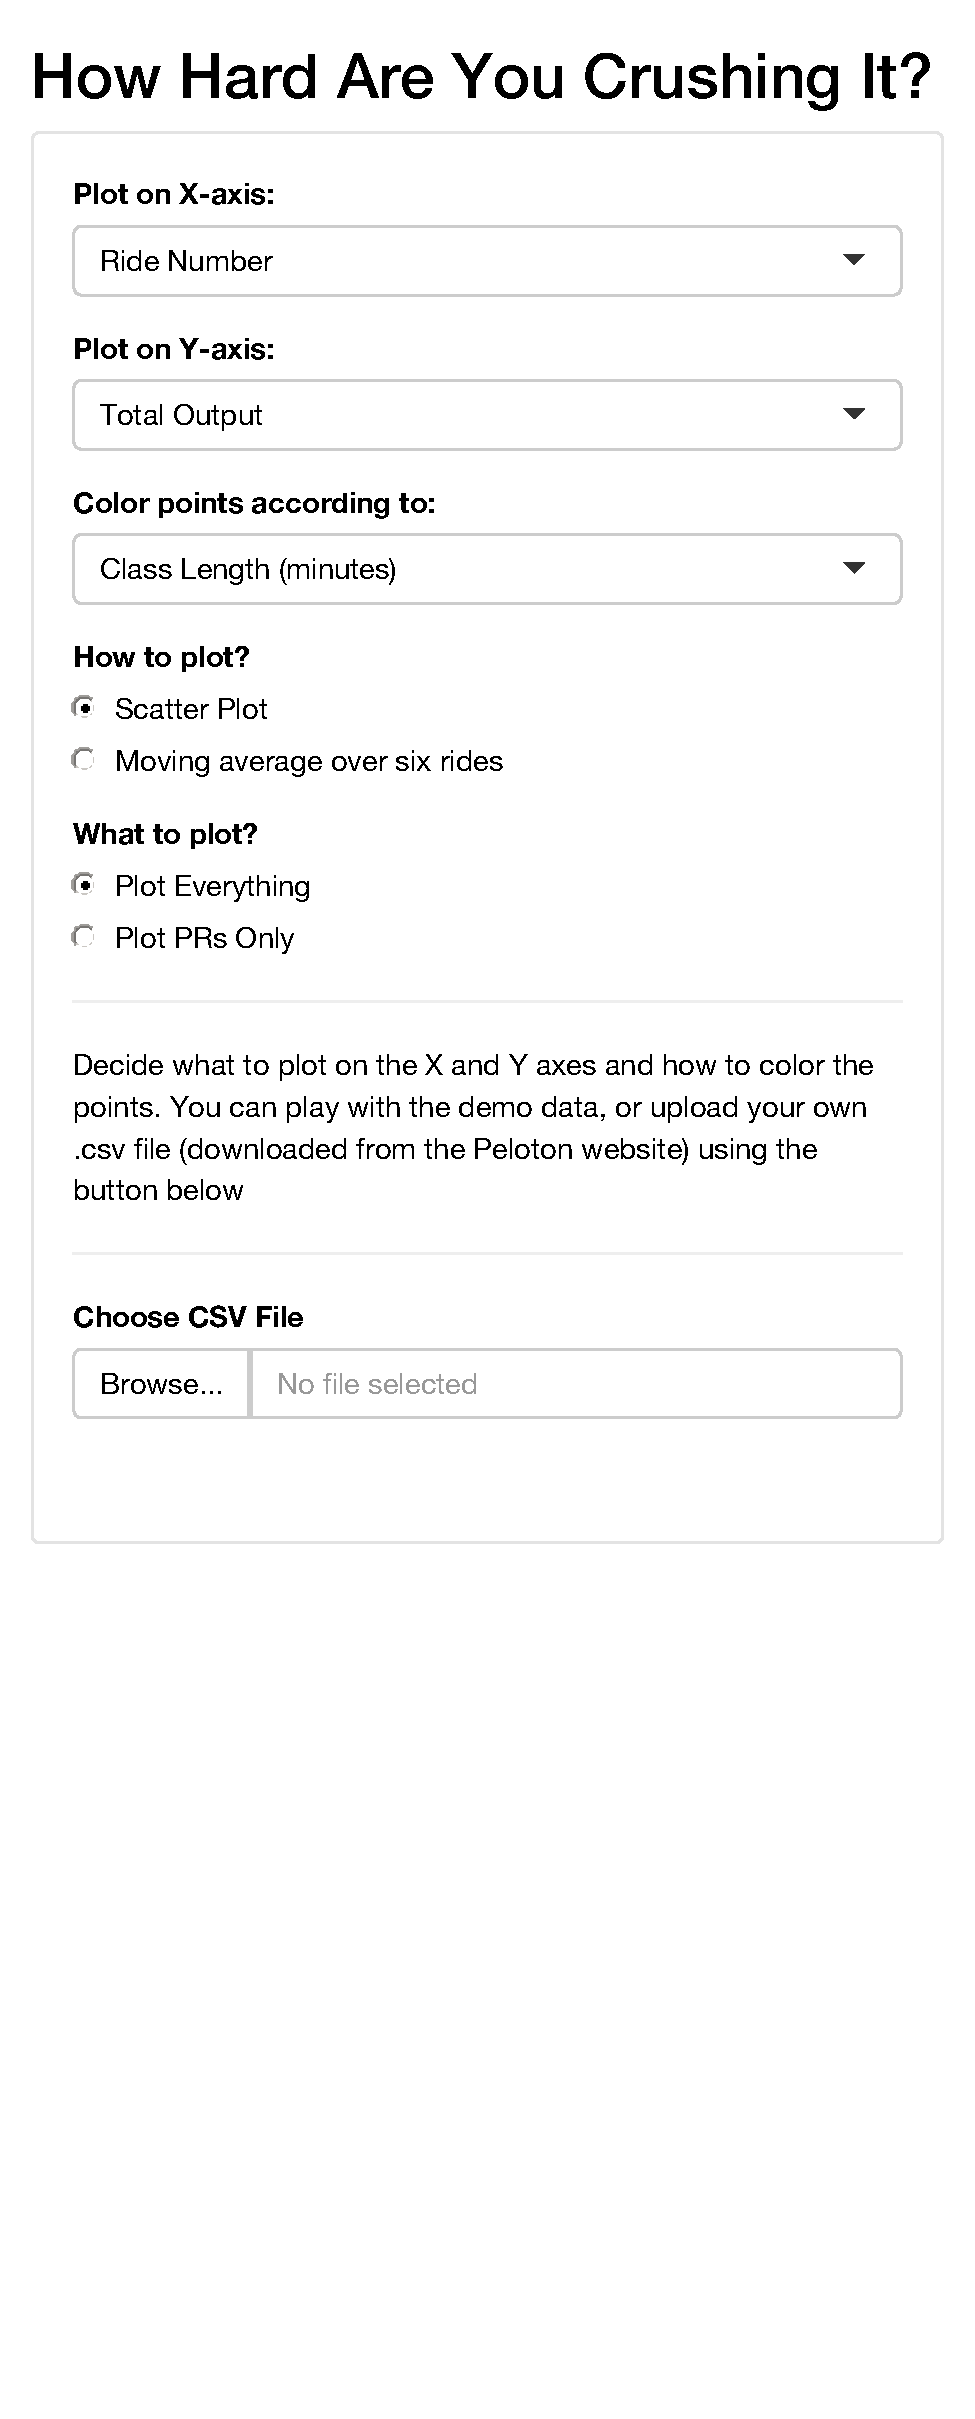
\includegraphics{GamifyingRides_files/figure-latex/Shiny App-1.pdf}}

\newpage

\hypertarget{results}{%
\section{Results}\label{results}}

This is where we can see the datasets visualized in graphs. The datasets are visualized per user to show each of the user's performance through time and was plotted to show continuous data from 2020 to 2022.

The first two graphs in \emph{Figure 1} shows the performance of User1(Persona 1) and User2(Persona2), depending on the class taken and the length of the class in minutes while the \emph{Total Output} is represented by the fill color. We can assume that total output is synonymous to the number of classes taken plus the performance , as the performance cannot be masured if there is no class taken. This Graph is performance based and tracks the total output where one can see the progress the user made. On Figure 1, for both Persona 1 and 2, we can see that the usage has been in bursts which shows that having the Bike+ alone does not increase user's motivation to go on it. The Bike+ was bought in August 2020 where the usage happened within the first couple months that can be related to the excitement of a newly purchased exercise machine. However, we see the usage getting less then dropping off at the end of 2020 and start of the year 2021 and we see this pattern happen throughout the dataset of 2020-2022. This shows how \textbf{Peloton} needs to put in the effort to sustain users motivation to keep using the Bike+. What can potentially happen is the user will completely lose interest and halt the monthly membership which can mean less business for the company. Since the company relies for internal motivation to go back on the Bike+ in order for the company to deploy it's motivational affordances, the company also needs to put external efforts such as email reminders to users about new and upcoming classes, tracking who their favourite instructors are and showing their upcoming classes and giving a monthly report summary of usage.

Another interesting information we can gather from the graphs are the type of classes often taken by the users and how they relate to how much they have sustained the workouts by class repetition. The common class both users take repeatedly are the \emph{Power Zone} classes. These classes can be considered as one of the hardest but users can train for to build strength. \textbf{Power Zones} according to Peloton \emph{is one of the most effective ways to level up your fitness when it comes to indoor cycling. It is a method of fitness training designed to have users working at seven different levels of exertions(or zones)}. (Peloton 2022b) These classes are coaching heavy where the users have to follow the instructors on when to increase their \emph{Cadence} and \emph{Resistance} to meet the zone requirements and needs to be sustained in a certain amount of time over a range of weeks with a promise of increase strength and endurance measured through a fitness test called \textbf{Functional Threshold Power Test} or \textbf{FTP Test}. Users can also measure their progress by feeling for how much higher they can push their \emph{resistance} for. The higher the number their \emph{resistance} is, the more they have to push their pedals and will either have a high or low \emph{cadence} depending on how strong the users have become. Inspired by the users ability to meet and sustain certain power zones, the users can measure their own progress. It is worth noting that \textbf{Peloton} uses the word training or train in a lot of their classes. This is to further the identity the company wishes to cultivate in their users and that is their ability to perform better and see progress which leads to increase in motivation to keep working out. Another interesting data we can gather from the graph is how Music and Theme rides were also prominent classes the users are taking. Both the classes are Music inspired and something Peloton tries to invest in too. \textbf{Peloton} is known to add new artists and playlist as part of their classes. This is also based on user information as Peloton gives users ability to \emph{like} a song by tapping the heart beside it when it's playing in a class. Lastly, it is important to note that the Lane Break data is not part of this dataset as it is a new feature where Peloton shows a video game interface that looks like a race track where the user is asked to meet specific performance markers such as Cadence and Resistance to get points. Although the feature is available, the dataset is not available for download just yet.

\includegraphics{GamifyingRides_files/figure-latex/Graph Set 1 code-1.pdf} \includegraphics{GamifyingRides_files/figure-latex/Graph Set 1 code-2.pdf}

The following graphs visualizes both of the users performance per instructor and class type. This is also an interesting data to understand as Peloton invests in their instructors and they play a big role in promoting the motivational affordances built in to the system. Peloton has 16 instructors listed in the graph but does not include other instructors for non-cycling classes. The author believes that Peloton has this much number of instructors so users don't get bored of taking the same kind of classes and to also cater to different personalities. There are instructors who are know to have very difficult classes such as Alex Toussaint while some classes are know for the therapeutic approach of an instructor that talks about inspiring life lessons as her coaching practice. Based from the graphs we can see that there are instructors users commonly follow and prefer. The more circles there are, the more classes the users have taken with the same instructor. This data along with the type of class the users usually take based on the color of the circles may communicate the type of personality the users have. If \textbf{Peloton} takes this data, they can assume that user1 is likely to stick to classes that can help train for strength and endurance. Paying attention to the color of the circles, one can see that classes taken with Matt Wilpers, Olivia Amato and Denis Morton etc. were helping the user build for strength and endurance as the color indicates power zone classes. It is also interesting to see that User1 has Music based classes with two instructors which can tell us that the music played in these classes may be the users preference. This can also mean that the user resonates with the instructor and may find them relatable or fun to train with. Meanwhile we can see that the graph for User 2 shows a specific theme which is heavy on both music and theme rides. These rides are often harder than it seems, it is usually dependent on who the instructor is. We see that Ally Love and Alex Toussaint were the user's top instructors based from how many circles there are and it can also show how well the users performance is improving as it is also showing increase in output. Understanding these two graphs help us understand why \textbf{Peloton} would invest in their instructors. The users need a coach to help them understand their performance and also to encourage them during difficult rides. In a business perspective, we can also assume that this is another way Peloton can gauge who the instructors they will retain based on how many classes users take with them. This can also be a source of motivation for the instructors to carefully curate their classes to inspire motivation and improve user performance.

\includegraphics{GamifyingRides_files/figure-latex/Graph Set 2 Code-1.pdf} \includegraphics{GamifyingRides_files/figure-latex/Graph Set 2 Code-2.pdf}

Understanding how each metric relates to the data extracted and how that can help us understand how the users performance is directly related to the motivational affordances the company designed for its users, let's have a quick overview of the summary of cycling classes for the users. As shown in the table below we can see that User 2 worked out significantly more than User 1. This means that between the two users, User 2 is more likely to respond to the motivational affordances around the experience and may be more metric centered. However, we also see that despite having less output, User 1 is still able to workout and sustain them for periods of time which can mean that there is no competition between the two users. This then tells us that \textbf{Self-competition} manifests through the numbers of output users have without having to relate to each others performance. We can assume that the performances the users have shown based on their data was purely from their own motivation that is either enhanced or elicited by the company's deliberate user experience design. \emph{Self-competition} then is a by product of the motivational affordances Peloton designed for and can be measured as total number of output per user. The higher the output is from the user the more self-competition manifests and fostered through the classes they take. It is worth noting that we can also measure self-competition based on user performance when riding based on leaderboard rankings, however, since there is no extractable way to get these data, we can only assume that the leaderboard rankings can improve performance. According to the users, they often do not engage with the leaderboard setting and usually removes it from the screen. However, the leaderboard feature is one of the first feature Peloton has and has kept which may mean that this function does elicit performance and may be the case for other users. Moreover, we can also assume that the Lane Break feature Peloton has recently added cultivates the idea of \emph{self-competition} as the user can gauge their performance by earning power points without having to ride with other users.

\begin{table}[!h]

\caption{(\#tab:Table 1)User Total Cycling Workout Summary 2020-2022}
\centering
\begin{tabular}[t]{lllll}
\toprule
User & Year\_2020 & Year\_2021 & Year\_2023 & Total\_Workout\\
\midrule
\cellcolor{gray!6}{Persona 1} & \cellcolor{gray!6}{25} & \cellcolor{gray!6}{122} & \cellcolor{gray!6}{30} & \cellcolor{gray!6}{177}\\
Persona 2 & 89 & 230 & 61 & 380\\
\bottomrule
\end{tabular}
\end{table}
\newpage

\hypertarget{discussion}{%
\section{Discussion}\label{discussion}}

\textbf{Gamification} has been increasingly popular as a design feature in the last couple of years. According to Bruhlman et al, paper on the effects of individual gamification elements on intrinsic motivation and performance, the attempts to apply games' motivational potential to various non-gaming context might foster user engagement.(Florian Bruhlmann 2017) As defined by Deterding et al, \textbf{Gamification} is the use of game design elements in non-game contexts.(Deterding et al. 2011) Nowadays, it is even utilized by social media applications where users are rewarded with a point system based from their content engagement. These points have monetary value as it can be used to pay for transactions at participating retailers.This reward practice is most commonly associated with gamification through the use of points, levels and leaderboards which may promote user behavior in various contexts.Seaborn and Fels (2015) However, several research cautioned on the over reliance on these game elements as it may diminish the intrinsic interest of the user that may lead to less engagement.Seaborn and Fels (2015) However, it is also argued that a well thought out implementation of game elements may improve intrinsic motivation by satisfying users' innate psychological needs for autonomy, competence and relatedness.Deterding (2014) Deterding further suggests that in order to understand the psychological mechanisms underlying gamification, the effects of individual game design elements on user motivation should be studied.(\textbf{Deterding2011?}) In a paper that Ping Zhang wrote on reasons information and communication design technology uses, he discusses the concept of \textbf{Motivational Affordance}. He defines this to be the properties of an object that determine whether and how these affordances affect one's motivational needs.Zhang suggests that direction implies that behavior has purpose, ``aimed or guided toward achieving some particular goal or avoiding some particular situations.'' (Zhang 2008) This is an interesting take on affordances and a thoughtful use of design to create an outcome. Affordance is a very common concept in \emph{User Experience Design} and is considered a design principle. Affordance is described as the actionable properties between the object and an actor/user. (Norman 1999) There are many examples of affordances and a common one would be the handle of a mug. What is interesting about affordance is it may not always be obvious to the user whether the action they are taking was designed to have the outcome or not. Zhang suggests that using a technology that satisfies motivational needs elicits enjoyment thus wanting more. This then becomes the ultimate goal of the design, to achieve motivational affordance so that users would be inclined to not just use it but also believe they cannot live without it. (Zhang 2008)

Emanuel Hurych best describes the term \textbf{Self-competition} in his paper discussing \emph{Self-Competition Versus Internal Competition} as competing with oneself. In his paper he describes self-competition to be based on accepting a challenge. He says that it could be a very important motive for a person to reach a chosen point and prepare for it, he even uses the sport Triathlon as an example.(Hurych 2009) This is interesting to note as \emph{triathletes do not compete with rivals but rather with time}. This is what Hurych believes to be a great example of self-competition or self-reflexive competition. Understanding the occurrence of self-competition, the author believes that the same experience is elicited by the \emph{motivational affordances} Peloton designed into their system. Based from our gathered data, we can see that both users have significantly made progress based from the increase in their \emph{Total Output} over a period of 3 months without needing to constantly participate in live classes or challenges that allows for inter-user competition during rides. Just like the triathletes in competition with time and their past performance, the users emulate the same. Self-competition then becomes an integral part of Peloton's artillery of features to utilize to keep the users coming back. When a user is motivated by their own performance and progress, users are more likely to follow through with more classes which then in turn become more business for Peloton as the user will continue to extend their membership. This shows how user \textbf{Self-Competition} is a by product of Peloton's \textbf{Motivational Affordances}. However, this is not sufficient enough to sustain a business model based on user engagement. Based from the sporadic workouts the users have in a span of almost two years, the users have only worked out with the Peloton in total of 378-9 each. This may mean that despite the efforts of the company to continue to build user engagement by motivating them through improving their performance, it's not enough to hold users attention and does not translate to commitment.

\hypertarget{data-strengths-and-weaknesses}{%
\subsection{Data Strengths and Weaknesses}\label{data-strengths-and-weaknesses}}

One of the biggest weakness of the datasets were the limited sample of user data. The user data is only accessible through an active users account, and because the author is only able to access two datasets, the information may not speak for users with different performance outcomes. These dataset are only able to draw conclusions based on two users. However, the author argues that despite the lack in user sample size, there is enough data gathered in over two years to make significant analysis on. The author also believes that the dataset contains a lot of relevant user information to be able to draw many different analysis and can be utilized in many ways even for just one user data. The data Peloton gathers from their user is relevant to their business and product research that one user data can be analyzed for different purposes. The report focused on just the cycling data which is only one aspect of the work outs that can be done with Peloton. This report also does not include data on newly released features such as the \textbf{Lane Break} which is the \emph{Video Game} simulated rides recently released on the Bike+ that furthers the \emph{gamification} of their rides. There is also a new hardware released by the company meant to track users performance through a camera that has an AI to assist users in strength training classes. If there is anything Peloton is good at, it's their ability to hone in on their user personas to create more features catering to assumed needs their users have. Peloton's success relies on their users attention and the longer they can hold the attention the longer they can stay in the game, be it through \emph{novelty of new hardware and features or invisible user experience design}.

\hypertarget{next-steps-and-conclusion}{%
\subsection{Next Steps and Conclusion}\label{next-steps-and-conclusion}}

The author hopes to continue to analyze the user performance data, and to include more of the newly integrated features to base the analysis on. It would be interesting to know how the performance differs for the Lane Break outputs or if it yields similar results and how that influences Peloton's decision on what feature and experience to create. It would also be interesting to study in-depth the performance data on Music based classes. Music is also an experience that can be designed and can elicit emotions or reactions and would be fascinating to see the data on how that can translate to user performance. The author also hopes that a survey can be done to gather more user experience data from users to compare with their own performance data. Overall the author believes that the user experience being designed for the intended user of Peloton Bike+ is not harmful to the user. It can enhance the user's physical activity which then leads to a more active and healthier body. It can also improve strength and endurance which can benefit the user's health and over all well-being.

In conclusion, Peloton's deployment of meticulous user experience design through motivational affordances does elicit an increase in user performance and motivation. Through the use of performance metrics and user performance encouragement by instructors, Peloton is able to draw out self-competition which evokes further motivation to increase work outs therefore continuing the membership for classes. Peloton can see and understand their users through the tracking of user information and can help the company address user needs and wants to build better personas that would fit the identity Peloton users have. This creates more loyalty to the brand and sustained membership over the long term.

\newpage

\appendix

\hypertarget{appendix}{%
\section*{Appendix}\label{appendix}}
\addcontentsline{toc}{section}{Appendix}

\textbf{Shiny App Link} - {]}Crushing It{]} (\url{https://arraycgh.shinyapps.io/crushing_it/})

\textbf{Gamification} - The use of games in none gaming environments to motivate users in applications or software as a service.(Deterding et al. 2011)

\textbf{Bike+} - Peloton's second version of their stationary indoor Bike.

\textbf{Leaderboard} - Peloton's built in active user ranking that rates users according to real-time performance.

\textbf{Watts} - Is defined as how much power you are exerting at any point in time. One can increase output by increasing \emph{cadence}, \emph{resistance} or both. (Peloton 2022c)

\textbf{Cadence} - Is how fast one pedals and is measured in RPMs or rotations per minute.(Peloton 2022c)

\textbf{Resistance} - Is the level of difficulty measured by percentage of the maximum resistance (0-100 percent). Resistance can be set by turning the red knob on the Bike+ to the right to increase it and to the left to decrease it.(Peloton 2022c)

\textbf{Output} - Is measured in Watts and can be used interchangeably. Watts is defined as how much power you are exerting at any point in time.(Peloton 2022c)

\textbf{Total Output} - measure in Kilojoules or KJ, is how much work the user has done over the whole ride. This is calculated by taking the average output times the number of seconds in the ride divided by 1,000.(Peloton 2022c)

\textbf{Persona} - Is a fictional, yet realistic description of a typical or target user of the product.(Harley 2015)

\textbf{Affordance} - Refer to the actionable properties between the world and an actor (a person or animal). (Gibson, Shaw, and Bransford 1977)

\textbf{Motivational Affordance} - Comprise of properties of an object that determine whether and how it support one's motivational needs.(Zhang 2008)

\textbf{Self-Competition} - Competition within oneself, is based on accepting a challenge. It could be a very important motive for a person to reach a chosen point and prepare for it. (Hurych 2009)

\newpage

\hypertarget{references}{%
\section*{References}\label{references}}
\addcontentsline{toc}{section}{References}

\hypertarget{refs}{}
\begin{CSLReferences}{1}{0}
\leavevmode\vadjust pre{\hypertarget{ref-Reddit2015}{}}%
2015. \emph{Reddit}. \url{https://www.reddit.com/r/pelotoncycle/comments/ccp18e/show_me_the_data_part_ii/}.

\leavevmode\vadjust pre{\hypertarget{ref-Deterding2014}{}}%
Deterding, Sebastian. 2014. {``Eudaimonic Design, or: Six Invitations to Rethink Gamification.''}

\leavevmode\vadjust pre{\hypertarget{ref-DeterdingEtal2011}{}}%
Deterding, Sebastian, Dan Dixon, Rilla Khaled, and Lennart Nacke. 2011. {``From Game Design Elements to Gamefulness: Defining" Gamification",''} 9--15.

\leavevmode\vadjust pre{\hypertarget{ref-PelotonBike}{}}%
{``Exercise Bike with Indoor Cycling Classes Streamed Live \& on-Demand\_2022.''} 2022. \emph{@Onepeloton}. \url{https://www.onepeloton.ca/bikes}.

\leavevmode\vadjust pre{\hypertarget{ref-Janitor}{}}%
Firke, Sam. 2021. \emph{Janitor: Simple Tools for Examining and Cleaning Dirty Data}. \url{https://CRAN.R-project.org/package=janitor}.

\leavevmode\vadjust pre{\hypertarget{ref-BruhlmannEtal2017}{}}%
Florian Bruhlmann, Alexander Tuch, Elisa Mekler. 2017. {``Towards Understanding the Effects of Individual Gamification Elements on Intrinsic Motivation and Performance.''} https://doi.org/\url{https://doi.org/10.1016/j.chb.2015.08.048}.

\leavevmode\vadjust pre{\hypertarget{ref-Francisco2013}{}}%
Francisco-Aparicio, Andrés, Francisco Luis Gutiérrez-Vela, José Luis Isla-Montes, and José Luis González Sanchez. 2013. {``Gamification: Analysis and Application.''} In \emph{New Trends in Interaction, Virtual Reality and Modeling}, 113--26. Springer.

\leavevmode\vadjust pre{\hypertarget{ref-JJGibson}{}}%
Gibson, James J, Robert Shaw, and John Bransford. 1977. \emph{Perceiving, Acting, and Knowing: Toward an Ecological Psychology}. Erlbaum, NJ.

\leavevmode\vadjust pre{\hypertarget{ref-Hamari2014}{}}%
Hamari, Juho, Jonna Koivisto, and Harri Sarsa. 2014. {``Does Gamification Work?--a Literature Review of Empirical Studies on Gamification,''} 3025--34.

\leavevmode\vadjust pre{\hypertarget{ref-NielsenNormanGroup}{}}%
Harley, Aurora. 2015. {``Personas Make Users Memorable for Product Team Members.''} \url{https://www.nngroup.com/articles/persona/}.

\leavevmode\vadjust pre{\hypertarget{ref-Glue}{}}%
Hester, Jim, and Jennifer Bryan. 2022. \emph{Glue: Interpreted String Literals}. \url{https://CRAN.R-project.org/package=glue}.

\leavevmode\vadjust pre{\hypertarget{ref-Hurych2009}{}}%
Hurych, Emanuel. 2009. {``Self-Competition Versus Internal Competition.''} \emph{ResearchGate}. De Gruyter Open Sp. z o.o. \url{https://www.researchgate.net/publication/243754950_Self-competition_versus_Internal_Competition}.

\leavevmode\vadjust pre{\hypertarget{ref-GT}{}}%
Iannone, Richard, Joe Cheng, and Barret Schloerke. 2022. \emph{Gt: Easily Create Presentation-Ready Display Tables}. \url{https://CRAN.R-project.org/package=gt}.

\leavevmode\vadjust pre{\hypertarget{ref-BastanfardEtal2018}{}}%
Mohammad Hajarian, Javad Mohammadzadeh, Azam Bastanfard. 2018. {``A Personalized Gamification Method for Increasing User Engagement in Social Networks.''} https://doi.org/\url{https://doi.org/10.1007/s13278-019-0589-3}.

\leavevmode\vadjust pre{\hypertarget{ref-Norman1999}{}}%
Norman, Donald A. 1999. {``Affordance, Conventions, and Design.''} \emph{Interactions} 6 (3): 38--43.

\leavevmode\vadjust pre{\hypertarget{ref-Peloton-Watts}{}}%
Peloton. 2022a. {``How the Peloton Bike Calculates Power Output (Watts).''} \url{https://support.onepeloton.com/hc/en-ca/articles/208776926-How-The-Peloton-Bike-Calculates-Power-Output-Watts-}.

\leavevmode\vadjust pre{\hypertarget{ref-Peloton-PowerZone}{}}%
---------. 2022b. {``Maximize Your Workouts: Power Zone Training FAQs.''} \url{https://blog.onepeloton.com/power-zone-training-faqs-with-matt-wilpers-and-denis-morton/}.

\leavevmode\vadjust pre{\hypertarget{ref-Peloton-Metrics}{}}%
---------. 2022c. {``Understanding Your Metrics.''} \url{https://support.onepeloton.com/hc/en-ca/articles/203325985-Understanding-your-metrics}.

\leavevmode\vadjust pre{\hypertarget{ref-citeR}{}}%
R Core Team. 2020. \emph{R: A Language and Environment for Statistical Computing}. Vienna, Austria: R Foundation for Statistical Computing. \url{https://www.R-project.org/}.

\leavevmode\vadjust pre{\hypertarget{ref-Seaborn2015}{}}%
Seaborn, Katie, and Deborah I Fels. 2015. {``Gamification in Theory and Action: A Survey.''} \emph{International Journal of Human-Computer Studies} 74: 14--31.

\leavevmode\vadjust pre{\hypertarget{ref-Ggplot2}{}}%
Wickham, Hadley. 2016. \emph{Ggplot2: Elegant Graphics for Data Analysis}. Springer-Verlag New York. \url{https://ggplot2.tidyverse.org}.

\leavevmode\vadjust pre{\hypertarget{ref-Tidyverse}{}}%
Wickham, Hadley, Mara Averick, Jennifer Bryan, Winston Chang, Lucy DAgostino McGowan, Romain François, Garrett Grolemund, et al. 2019. {``Welcome to the {tidyverse}.''} \emph{Journal of Open Source Software} 4 (43): 1686. \url{https://doi.org/10.21105/joss.01686}.

\leavevmode\vadjust pre{\hypertarget{ref-Dplyr}{}}%
Wickham, Hadley, Romain François, Lionel Henry, and Kirill Müller. 2021. \emph{Dplyr: A Grammar of Data Manipulation}. \url{https://CRAN.R-project.org/package=dplyr}.

\leavevmode\vadjust pre{\hypertarget{ref-TidyR}{}}%
Wickham, Hadley, and Maximilian Girlich. 2022. \emph{Tidyr: Tidy Messy Data}. \url{https://CRAN.R-project.org/package=tidyr}.

\leavevmode\vadjust pre{\hypertarget{ref-Readr}{}}%
Wickham, Hadley, Jim Hester, and Jennifer Bryan. 2022. \emph{Readr: Read Rectangular Text Data}. \url{https://CRAN.R-project.org/package=readr}.

\leavevmode\vadjust pre{\hypertarget{ref-Zhang2008}{}}%
Zhang, Ping. 2008. {``Motivational Affordances: Reasons for ICT Design and Use.''} \emph{Communications of the ACM} 51 (11): 145--47.

\leavevmode\vadjust pre{\hypertarget{ref-KableExtra}{}}%
Zhu, Hao. 2021. \emph{kableExtra: Construct Complex Table with 'Kable' and Pipe Syntax}. \url{https://CRAN.R-project.org/package=kableExtra}.

\end{CSLReferences}

\end{document}
